\documentclass{beamer}

\usepackage{multirow}
\usepackage{pgfplots}

\pgfplotsset{compat=1.17}

\mode<presentation>
{
    \usetheme{Warsaw}
}

\title{CycleMLP}
\subtitle{A MLP-like Architecture for Dense Prediction}
\author{Marco Benelli}
\institute{University of Florence}
\date{February 14, 2022}

\DeclareMathOperator{\layernorm}{LayerNorm}

\begin{document}

\begin{frame}
    \titlepage
\end{frame}

\begin{frame}{Outline}
    \tableofcontents
\end{frame}

\section{Introduction}

\begin{frame}{Paradigm Shifts}
    Recent paradigm shifts:
    \begin{description}
        \item[2012] AlexNet
        \item[2020] ViT
        \item[2021] MLP-Mixer
    \end{description}
\end{frame}

\begin{frame}{MLP-Mixer}
    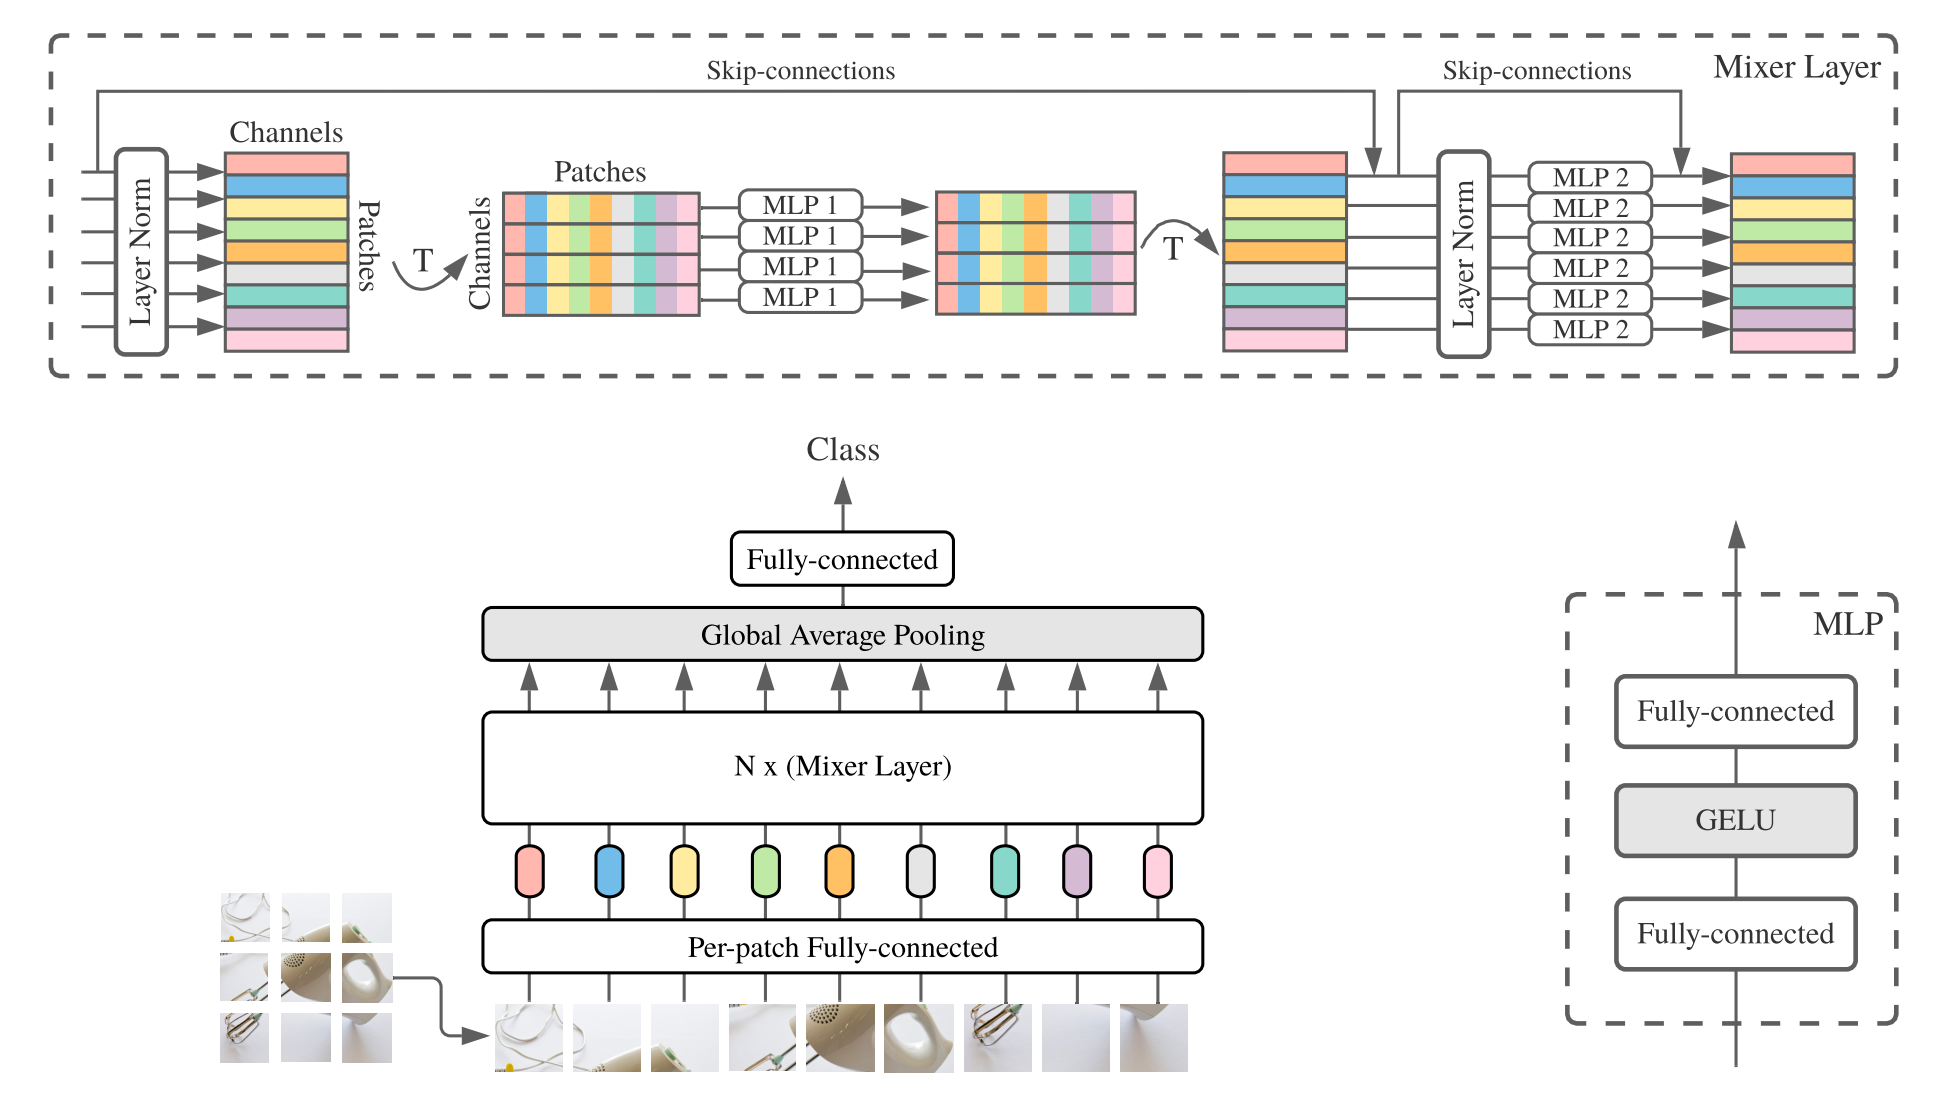
\includegraphics[width=\textwidth]{figures/mixer_figure.png}
\end{frame}

\begin{frame}{Mixer Layer}
    $$\mathbf{U}_{*,i} = \mathbf{X}_{*,i} + \mathbf{W}_2 \sigma(\mathbf{W}_1 \layernorm(\mathbf{X})_{*,i}), \quad \text{for } i = 1 \dots C$$
    $$\mathbf{Y}_{j,*} = \mathbf{U}_{j,*} + \mathbf{W}_4 \sigma(\mathbf{W}_3 \layernorm(\mathbf{U})_{j,*}), \quad \text{for } j = 1 \dots S$$
\end{frame}

\begin{frame}{Challenges}
    MLP-like models are facing these challenges:
    \begin{itemize}
        \item non-hierarchical architectures
        \item flexible input scales
        \item quadratic costs
    \end{itemize}
\end{frame}

\section{Method}

\subsection{Cycle Fully-Connected Layer}

\begin{frame}{Cycle FC}
    \centering
    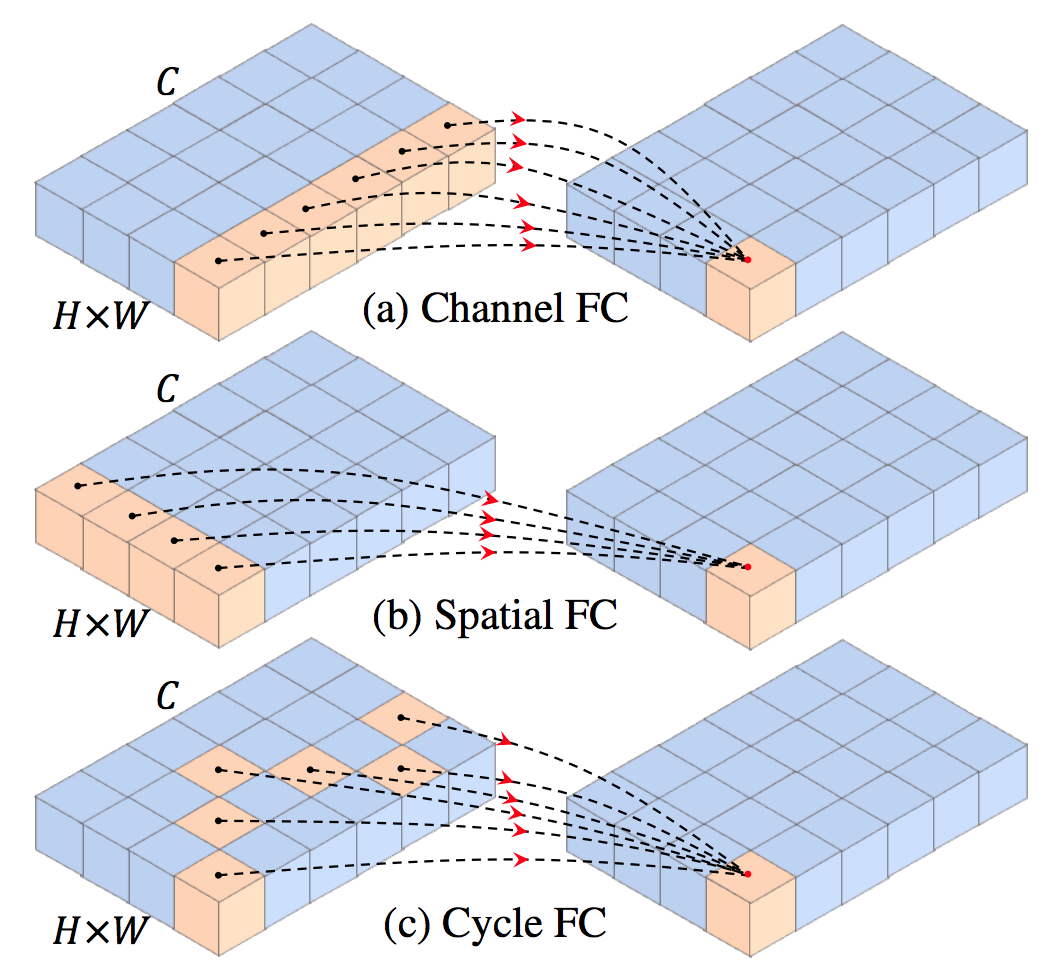
\includegraphics[height=.8\textheight]{figures/teaser.png}
    % \parbox{.4\textwidth}{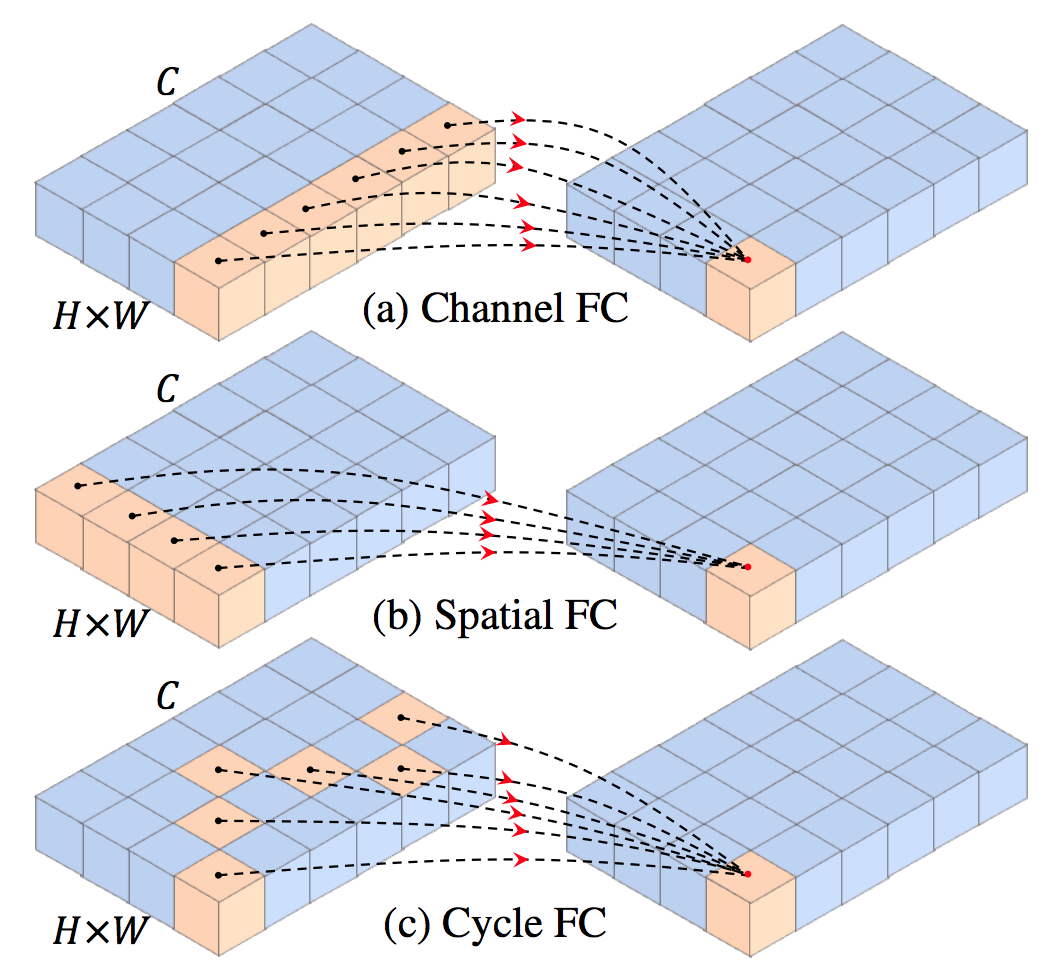
\includegraphics[width=.4\textwidth]{figures/teaser.png}}
    % \parbox{.4\textwidth}{\begin{tabular}{c c c}
    %     \hline
    %     FC & $\mathcal{O}(HW)$ & \begin{tabular}{c}Scale \\ Variable\end{tabular} \\
    %     \hline
    %     Channel & $HW$ & Yes \\
    %     \hline
    %     Spatial & $H^2W^2$ & No \\
    %     \hline
    %     Cycle & $HW$ & Yes \\
    %     \hline
    % \end{tabular}}
\end{frame}

\begin{frame}{Stepsize Example}
    \centering
    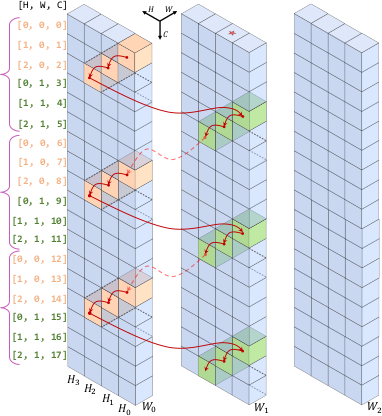
\includegraphics[height=.8\textheight]{figures/stepsize_3_2.png}
\end{frame}

\subsection{Overall Architecture}

\begin{frame}{Comparison Of MLP Blocks}
    \centering
    \parbox{.4\textwidth}{\centering 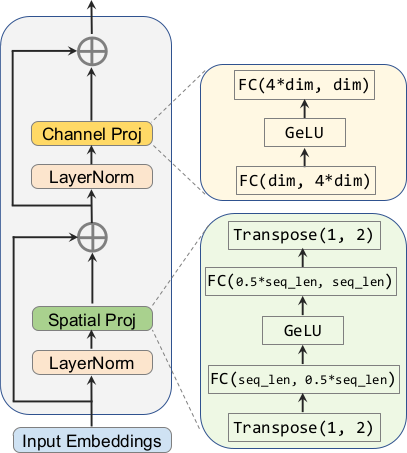
\includegraphics[width=.4\textwidth]{figures/block_mlpmixer.png}}
    \parbox{.4\textwidth}{\centering 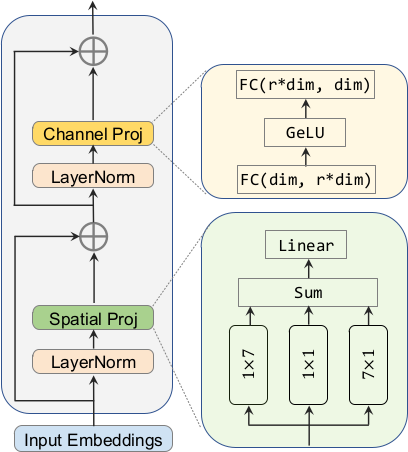
\includegraphics[width=.4\textwidth]{figures/block_cyclemlp.png}}
\end{frame}

\begin{frame}{Hierarchy}
    \centering
    \parbox{.4\textwidth}{\centering 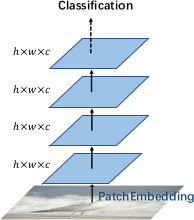
\includegraphics[width=.4\textwidth]{figures/hierarchy_singlestage.png}}
    \parbox{.4\textwidth}{\centering 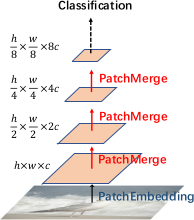
\includegraphics[width=.4\textwidth]{figures/hierarchy_pyramid.png}}
\end{frame}
\begin{frame}{Instantiation}
    \centering
    \resizebox{!}{.4\textheight}{\begin{tabular}{c|c|c|c}
        \hline
        & Output Size & Layer Name & B1 \\
        \hline
        \multirow{2}{*}{Stage 1} & \multirow{2}{*}{$\frac{H}{4} \times \frac{W}{4}$}
            & \begin{tabular}[c]{@{}c@{}} Overlapping \\ Patch Embedding \end{tabular} & $C_1=64$ \\
            \cline{3-4} 
            & & \begin{tabular}[c]{@{}c@{}} CycleMLP \\ Block \end{tabular} & \begin{tabular}[c]{@{}c@{}} $E_1=4$ \\ $L_1=2$ \end{tabular} \\
        \hline
        \multirow{2}{*}{Stage 2} & \multirow{2}{*}{$\frac{H}{8} \times \frac{W}{8}$}
            & \begin{tabular}[c]{@{}c@{}} Overlapping \\ Patch Embedding \end{tabular} & $C_2=128$  \\
            \cline{3-4} 
            & & \begin{tabular}[c]{@{}c@{}} CycleMLP \\ Block \end{tabular} & \begin{tabular}[c]{@{}c@{}} $E_2=4$ \\ $L_2=2$ \end{tabular} \\
        \hline
        \multirow{2}{*}{Stage 3} & \multirow{2}{*}{$\frac{H}{16} \times \frac{W}{16}$}
            & \begin{tabular}[c]{@{}c@{}} Overlapping \\ Patch Embedding \end{tabular} &  $C_3=320$ \\
            \cline{3-4} 
            & & \begin{tabular}[c]{@{}c@{}} CycleMLP \\ Block \end{tabular} & \begin{tabular}[c]{@{}c@{}} $E_3=4$ \\ $L_3=4$ \end{tabular} \\
        \hline
        \multirow{2}{*}{Stage 4} & \multirow{2}{*}{$\frac{H}{32} \times \frac{W}{32}$}
            & \begin{tabular}[c]{@{}c@{}} Overlapping \\ Patch Embedding \end{tabular} & $C_4=512$ \\
            \cline{3-4} 
            & & \begin{tabular}[c]{@{}c@{}} CycleMLP \\ Block \end{tabular} & \begin{tabular}[c]{@{}c@{}} $E_4=4$ \\ $L_4=2$ \end{tabular} \\
        \hline
    \end{tabular}}
\end{frame}

\section{Classification Experiments}

\begin{frame}{Experimental Setup}
    \begin{itemize}
        \item optimizer AdamW
        \item $\lambda = 5 \times 10^{-2}$
        \item cosine annealing learning rate schedule
        \item $\eta_{\text{max}} = 1 \times 10^{-3}$
        \item $T_\text{max} = 100$
        \item $\text{batch size} = 256$
    \end{itemize}
\end{frame}

\begin{frame}{Experiments}
    \centering
    \begin{tabular}{c c c}
        \hline
        Model & STL10 & CIFAR10 \\
        \hline
        ResNet & 64.9\% & 77.1\% \\
        % RegNet & 51.5\% & 60.6\% \\
        ViT & 44.4\% & 53.4\% \\
        MLP-Mixer & 51.4\% & 55.5\% \\
        CycleMLP & 49.8\% & 66.5\% \\
        \hline
    \end{tabular}
\end{frame}

\subsection{CIFAR10}

\begin{frame}{Loss Plot (CIFAR10)}
    \centering
    \begin{tikzpicture}
        \begin{axis}[
            no markers,
            xlabel=epoch,
            ylabel=loss,
            legend pos=south west,
            % xmin=0, xmax=99,
            % ymin=0,
            ]
            \addplot table [x=epoch,y=train loss,col sep=comma] {tables/cifar10.csv};
                \addlegendentry{train}
            \addplot table [x=epoch,y=test loss,col sep=comma] {tables/cifar10.csv};
                \addlegendentry{test}
        \end{axis}
    \end{tikzpicture}
\end{frame}

\begin{frame}{Accuracy Plot (CIFAR10)}
    \centering
    \begin{tikzpicture}
        \begin{axis}[
            no markers,
            xlabel=epoch,
            ylabel=accuracy,
            legend pos=north west,
            % xmin=0, xmax=99,
            ymin=0, % ymax=1,
            ]
            \addplot table [x=epoch,y=train accuracy,col sep=comma] {tables/cifar10.csv};
                \addlegendentry{train}
            \addplot table [x=epoch,y=test accuracy,col sep=comma] {tables/cifar10.csv};
                \addlegendentry{test}
        \end{axis}
    \end{tikzpicture}
\end{frame}

\subsection{STL10}

\begin{frame}{Loss Plot (STL10)}
    \centering
    \begin{tikzpicture}
        \begin{axis}[
            no markers,
            xlabel=epoch,
            ylabel=loss,
            legend pos=south west,
            % xmin=0, xmax=99,
            % ymin=0,
            ]
            \addplot table [x=epoch,y=train loss,col sep=comma] {tables/stl10.csv};
                \addlegendentry{train}
            \addplot table [x=epoch,y=test loss,col sep=comma] {tables/stl10.csv};
                \addlegendentry{test}
        \end{axis}
    \end{tikzpicture}
\end{frame}

\begin{frame}{Accuracy Plot (STL10)}
    \centering
    \begin{tikzpicture}
        \begin{axis}[
            no markers,
            xlabel=epoch,
            ylabel=accuracy,
            legend pos=north west,
            % xmin=0, xmax=99,
            ymin=0, % ymax=1,
            ]
            \addplot table [x=epoch,y=train accuracy,col sep=comma] {tables/stl10.csv};
                \addlegendentry{train}
            \addplot table [x=epoch,y=test accuracy,col sep=comma] {tables/stl10.csv};
                \addlegendentry{test}
        \end{axis}
    \end{tikzpicture}
\end{frame}

\subsection{ImageNet-1K}

\begin{frame}{ImageNet-1K Comparison}
    \centering
    \begin{tabular}{c c}
        \hline
        Model & Accuracy \\
        \hline
        ResNet & 69.8\% \\
        % RegNet & 81.7\% \\
        ViT & 77.9\% \\
        MLP-Mixer & 61.4\% \\
        CycleMLP & 79.1\% \\
        \hline
    \end{tabular}
\end{frame}

\section*{Summary}

\begin{frame}{Summary}
    \begin{itemize}
        \item CycleMLP is built upon the \alert{Cycle FC}.
        \item Cycle FC is capable of dealing with \alert{variable input scales}.
        \item The computational cost of Cycle FC is \alert{$O(HWC^2)$}.
    \end{itemize}
\end{frame}

\end{document}
